\chapter{Supplementary Results}
\label{app:results}

This appendix holds the full results behind the headline figures of Chapter~\ref{chap:results}: the run history of each test across firmware versions, the per-run and per-source breakdowns, and the longer tables. The sections follow that chapter, requirement by requirement; the raw evidence is indexed in Appendix~\ref{app:evidence}.

\section{Inertial acquisition (R1)}
\label{sec:resx-acq}

Table~\ref{tab:res-acquisition} summarises the acquisition results. Both IMUs held 200\,Hz with no dropped samples in every bench session, including with all subsystems running together on the target board. The only timing fault was the pause at each flash write. With a write every 10\,s (v0.5.0) both IMUs showed a 33 to 40\,ms gap at every write, twelve in two minutes; with logging switched off for the next two minutes the worst gap was 5.9\,ms. With buffered logging (v0.6.0), in a 330\,s run with five flushes, all ten gaps over 10\,ms (37 to 40\,ms, both IMUs at each flush) fell in the first statistics window reported after a flush, 0.2 to 1.05\,s after it (Figure~\ref{fig:res-imu-gaps}), and the worst gap elsewhere was again 5.9\,ms. Each flush occupied the modem task for 71 to 202\,ms, which does not affect acquisition. With v0.7.4 and its 94\,Hz filter the rate and drop count were unchanged (T15). ``No dropped samples'' does not mean even spacing: in the 25 September session the shortest interval fell to 0.8 to 1.0\,ms in each window with a write gap, as \texttt{vTaskDelayUntil} caught up, and jerk, computed with a fixed $\Delta t$, is distorted there. R1 is met on the bench as defined. The drop counter counts samples lost because the queue was full. Up to v0.7.4.1 a read that failed on the bus was not detected and passed as a sample, so those loss figures cover the processing path, not the bus; since v0.7.5 failed and stuck reads are counted (Section~\ref{sec:imu-health}).

\begin{table}[htbp]
\centering
\caption[Inertial acquisition on the target board (bench)]{Inertial acquisition on the target board (bench).}
\label{tab:res-acquisition}
\begin{tabular}{|p{6.2cm}|p{7.6cm}|}
\hline
\textbf{Measure} & \textbf{Result} \\ \hline
Sample rate, each IMU & 200.0 to 200.5\,Hz in every bench session \\ \hline
Dropped samples (queue full) & 0 in every bench session \\ \hline
Longest gap, logging off & 5.9\,ms; none over 10\,ms \\ \hline
Gap at each flash write, 25 Sep session & 24.8 to 29.9\,ms every 12\,s; shortest interval 0.8 to 1.0\,ms in the same windows (catch-up) \\ \hline
Gap at each flash write, v0.5.0 & 33 to 40\,ms, every 10\,s \\ \hline
Gap at each flash write, v0.6.0 (buffered) & 37 to 40\,ms, about once a minute, each in the first window after a flush \\ \hline
v0.7.4, 94\,Hz filter, 12-minute T15 run & 200.0 to 200.5\,Hz, 0 dropped in 736 windows; 36 to 44\,ms at each flush, none added by the replay \\ \hline
All subsystems together (IMUs, BLE, modem) & 400 to 401 samples per 2\,s window on each IMU, 0 dropped \\ \hline
Dashboard line added (v0.7.0) & 200\,Hz on both IMUs, 0 dropped \\ \hline
\end{tabular}
\end{table}

Figure~\ref{fig:res-imu-gaps} shows the longest sample interval in each 2\,s window. With v0.5.0 (29 September), 30 of the 151 logging-on windows per IMU had a maximum interval of 33.0 to 40.0\,ms, one about every 10\,s, and in the 59 windows with flash logging off the worst interval was 5.9\,ms. With buffered writes in v0.6.0 (1 October) only 5 of 173 windows per IMU exceeded 10\,ms (37.3 to 40.1\,ms), each in the first window reported after one of the five flushes, and the worst interval elsewhere was 5.9\,ms; no sample was dropped in either run.

On the first road session (19 October; Section~\ref{sec:field-test-design}), which included about 16 minutes of driving, the drop count stayed at zero on both IMUs throughout. The unit sends one record a second, but the recorder polled twice a second and the bridge repeated its last record until a new line arrived, so the 10,287 rear replies hold 3,464 distinct records. Over the 5,557\,s from the first to the last (17:16:37 to 18:49:13), 2,093 seconds (38\,\%) have no record, and in the driving period (18:15 to 18:49) 67\,\% of seconds have one. The missing seconds are lines lost between the unit and the Raspberry Pi~4 over USB, the loss already seen on the bench (R10 below), and 27 of the records that arrived had damaged fields. Of the 3,437 readable records, 3,431 show both IMUs at 200.0 to 200.5\,Hz; five, at 18:03 to 18:05, show 197 to 204.5\,Hz, an uneven split of samples between two-second windows; and one, at 18:29:16 while driving, shows IMU1 with 4 samples in a 2\,s window instead of 400, a stall of nearly 2\,s that the drop count does not show and whose cause is not known. On the vehicle R1 is therefore not met: the drop count stayed at zero and the rate held except for that stall, but a third of the per-second records did not reach the recorder.

On 21 and 22 October, with the unit on its own battery and its record on the wired link (Section~\ref{sec:pi-link}), the rear unit's drop counts rose at about 168 and 46 a second until a reset, while the reported rate stayed at 200\,Hz and the vibration value was null. The statistics and ride tasks had stopped on the IMU core; v0.7.6 moved them to the other core (Section~\ref{sec:inv-stall}). IMU2, not detected after one reset, was then moved to the front node. Table~\ref{tab:res-twonode} gives the bench results of 22 October on the two nodes.

\begin{table}[htbp]
\centering
\small
\caption[Bench results of 22 October 2026 on the front node and the rear unit (lab notebook, 22 October; soak in \texttt{Report/\allowbreak{}figures/\allowbreak{}results/\allowbreak{}soak\_\allowbreak{}v076b\_\allowbreak{}summary.txt})]{Bench results of 22 October 2026 on the front node and the rear unit (lab notebook, 22 October; soak in \texttt{Report/\allowbreak{}figures/\allowbreak{}results/\allowbreak{}soak\_\allowbreak{}v076b\_\allowbreak{}summary.txt}).}
\label{tab:res-twonode}
\begin{tabular}{|p{4.6cm}|p{9.2cm}|}
\hline
\textbf{Test} & \textbf{Result} \\ \hline
Front node raw stream to the laptop, v0.7.5 & At 115\,200\,baud: 5,110 samples in 20\,s, 0 missing, line 85\,\% full. At 921\,600\,baud: 6,800 samples in 30\,s, 0 missing by sequence, 0 bad lines, 69 sync edges, 0 raw drops \\ \hline
Front node on the Raspberry Pi~5 (capture service) & 200\,Hz, 0 drops, 0 read failures, 0 raw drops; 1,107 raw lines by 12:27 and 2,608 by 12:58, 0 bad CRC; recorder 80 of 80 polls of the front node. On v0.7.6: 200\,Hz, 0 drops, consumer ages 0 and 4\,ms, both cores idle \\ \hline
Front sync pulse & GPIO5 to Pi~5 pin~11 toggles every 500\,ms (rear pulse on the Raspberry Pi~4 since 30 September, Table~\ref{tab:res-camera}) \\ \hline
Rear unit after flashing v0.7.6 & IMU1 200\,Hz, 0 drops, 0 read failures, 0 late, highest queue fill 2, consumer ages 1, 2 and 45\,ms, vibration 0.026; raw stream saved on the Raspberry Pi~4, 0 bad CRC \\ \hline
Rear unit, IMU1 wires taken off while running (v0.7.6) & 17,080 read failures and 8,508 late slots, 0 drops, consumer ages 2 to 29\,ms, both cores idle; on refitting, the sensor repeated one reading (stuck rising 200 a second) until reset \\ \hline
Rear unit soak, v0.7.6, 62\,min (13:48 to 14:50), own battery, modem silent, wired UART & 0 restarts; 0 drops, 0 read failures, 0 raw drops, 0 late; highest queue fill 7; consumer ages at most 49\,ms; idle counts at least 976 and 1,597 a second on the two cores; vibration in every record (median 0.027\,m/s\textsuperscript{2}); IMU1 199.5 to 200.5\,Hz in 723 of 726 polls, 201.3 to 203.9 in three; 152 stuck readings; bridge 3,720 lines in 3,720\,s, 0 bad \\ \hline
\end{tabular}
\end{table}

The soak met every pass criterion of the v0.7.6 bench test (\texttt{TelemetryUnit/\allowbreak{}CHANGELOG.md}) except the rate, which was above 200.5\,Hz in 3 of 726 polls with no sample dropped or late. The 152 stuck readings, about 2 in 10,000 samples, came a few at a time (1 to 6) every 82 to 87\,s, on the period at which the 8\,kB log buffer is written to flash. Each write pauses the IMU task for about 40\,ms (Section~\ref{sec:res-acq}); the catch-up reads that follow come about 1\,ms apart, faster than the sensor's 1\,kHz update, so some repeat the previous value and are counted as stuck, and the same catch-up samples falling into the next 2\,s window explain the three high rates. They are far below the 200 in a row that triggers re-initialisation in v0.7.7, and logging to flash can be switched off (\texttt{!log off}) when the raw stream on the Raspberry Pis is the record. The fault had appeared after 23 to 45 minutes on a battery with the modem silent, and the soak ran 62 minutes under those conditions without it. The trigger was not reproduced on v0.7.4.1 first, however, so the soak shows that v0.7.6 ran through the fault's conditions, not that the trigger was present. R1 is met on both nodes on the bench.

\section{Calibration (R2)}
\label{sec:resx-cal}

Before calibration, the two IMUs on the development board read about 5.7\% above and 2.6\% below standard gravity at rest, about 8\% apart. The factors stored at their first calibration were 0.9773 and 0.9901, after which both read 9.80 to 9.81\,m/s\textsuperscript{2}, agreeing within measurement noise. The factors imply mean magnitudes at the moment of calibration of 10.03 and 9.90\,m/s\textsuperscript{2}, not the readings seen earlier that day, so the uncalibrated readings had shifted between sessions; the likely cause, not confirmed, is that the sensors were moved in between. On the target board the first boot measured 9.44 and 9.57\,m/s\textsuperscript{2} (factors 1.0390 and 1.0245), and with those factors a later session read median resting magnitudes of 9.93 and 10.10\,m/s\textsuperscript{2}, 1.3\% and 2.9\% above gravity. R2 was met immediately after calibration but not in the later session, which suggests that a single factor holds only for the orientation in which it was measured.

On the front node (Planning/calibration-record.md) the first boot stored a factor of 1.0036 (mean magnitude 9.7718\,m/s\textsuperscript{2}), and a recalibration with \texttt{!recal} from the Raspberry Pi~5 on 22 October gave 1.0035 (9.7729\,m/s\textsuperscript{2}), with the board still in the same position: the procedure repeats within 0.01\,\%. The raw counts at rest were 4,096.6, exactly 1.000\,g at the sensor's scale, and the noise was 0.004 to 0.007\,g per axis. The board lay at 49\textdegree\ from level, so the factor is valid only until it is mounted. The rear unit was not recalibrated on 22 October.

\section{Ride features and fusion (R3)}
\label{sec:resx-ride}

The feature self-test passed at every boot: RMS, peak-to-peak and crest factor of the synthetic sine were within 5\% of their analytical values. All five fusion self-tests passed. In a 150\,s recorded session (Figure~\ref{fig:recorded-session}) all 149 fused windows combined both sensors with a skew below 1\,ms (the log holds 222 fused lines, because a window can be printed by either sensor's task or both; each window is counted once). The planned disturbance, between 50 and 70\,s on audible cues, did not happen because the cues were not heard; the board was disturbed from about 75 to 128\,s instead, and the log is annotated to say so. While the board was still (the first 70\,s), the fused vibration level $\sigma$ had a median of 0.041\,m/s\textsuperscript{2} and a maximum of 0.067\,m/s\textsuperscript{2}; during the hand disturbance it rose to 9.35\,m/s\textsuperscript{2}, and the largest peak-to-peak amplitude in a window was 77.6\,m/s\textsuperscript{2}, within 1\,m/s\textsuperscript{2} of the $\pm 8\,g$ range, so that peak was probably clipped. The disagreement figure $D$ ranged from 0.00 to 1.68. In an earlier disturbance test both sensors rose together (peak-to-peak from about 0.2 to 18.4 and 10.2\,m/s\textsuperscript{2}, crest factor from about 1.01 to 2.17 and 1.43, jerk from about 8 to 160 and 162\,m/s\textsuperscript{3}) and decayed together, so the calibrated pair also tracked each other under motion, not only at rest. R3 is met. These results show that the features are computed and combined as designed; they do not show how the features respond to the road or the motor.

\begin{figure}[htbp]
\centering
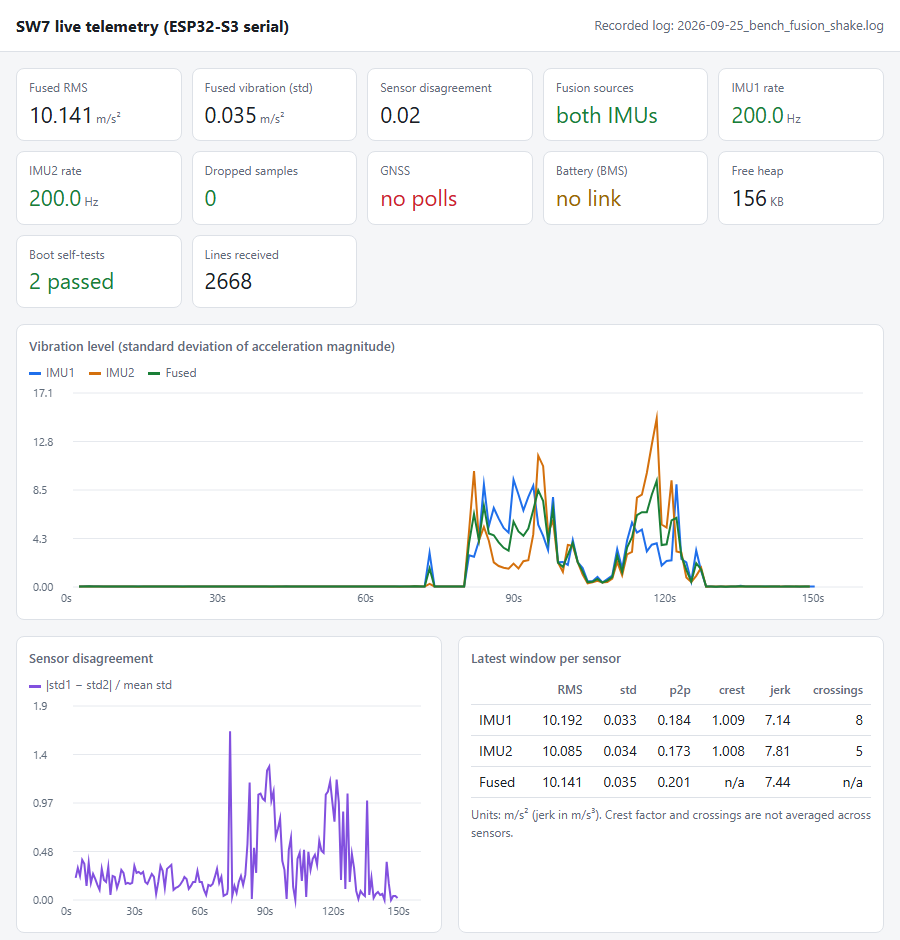
\includegraphics[width=0.6\textwidth]{figures/recorded_session.png}
\caption[A 150-second bench session recorded from power-up and replayed through the bench dashboard: still until about 75\,s, disturbed by hand until about 128\,s, then still again]{A 150-second bench session recorded from power-up and replayed through the bench dashboard: still until about 75\,s, disturbed by hand until about 128\,s, then still again.}
\label{fig:recorded-session}
\end{figure}

On the road session the per-second vibration value differed between the states, partly by construction, since a second was labelled by current or vibration. Counting each record once, and labelling a second as driving when the battery current exceeded 1\,A or the value exceeded 0.3, it had a median of 0.03 in the 2,832 parked seconds and, in the 605 driving seconds, a median of 1.39, a 95th percentile of 3.2 and a maximum of 5.09, with battery current of up to 46.9\,A. The full 1\,s features were stored only in the unit's own log (Section~\ref{sec:res-flashlog}), no raw samples were kept and the runs were not marked, so no per-run analysis is possible from this session.

Figure~\ref{fig:res-road} shows the 19 October session from the rear unit's telemetry. After removing repeats there were 3464 records between sequence numbers 4549 and 10105, so 2093 of 5557 (37.7\,\%) were not received: 407 in one gap from 18:06:34 to 18:13:23, the rest in short gaps of at most 8 records. Vibration stayed near 0.03\,m/s$^2$ (median 0.030) while parked and had a median of 1.39\,m/s$^2$ (maximum 5.09) in the 607 records flagged as driving (605 of them with every field readable), and the battery current reached $-46.9$\,A with a median of $-6.3$\,A over the 307 records above 1\,A.

\subsection{Run-1 flash log}
\label{sec:resx-flashlog}

The unit's own log of the session was read back on 22 October, before the unit was reflashed (\texttt{BenchTest/\allowbreak{}logs/\allowbreak{}flashlog\_\allowbreak{}2026-10-22/}): 2,000 of the 2,022 stored records after four passes, of which 1,998 parse; the other two had a bus error message printed into them during the read-back. Boot 109 (v0.7.4) holds the session: 1,154 records over 1.3 to 8.7\,h of uptime, which the recorder's records of the same boot place at 17:18 on 19 October to 00:44 on 20 October. Each record holds the battery state and, per IMU, the features of the latest 1\,s window (RMS, $\sigma$, peak-to-peak, crest factor, jerk), with the fused $\sigma$ and $D$. Records are meant to be 10\,s apart, but in this boot only 553 of 1,139 intervals were 10\,s and the rest up to 58\,s (mean 23\,s), so the log holds about one second in 23. The record is built in the modem task, which was also retrying MQTT with no broker reachable; that this stretched the interval is likely but not confirmed.

\begin{figure}[htbp]
\centering
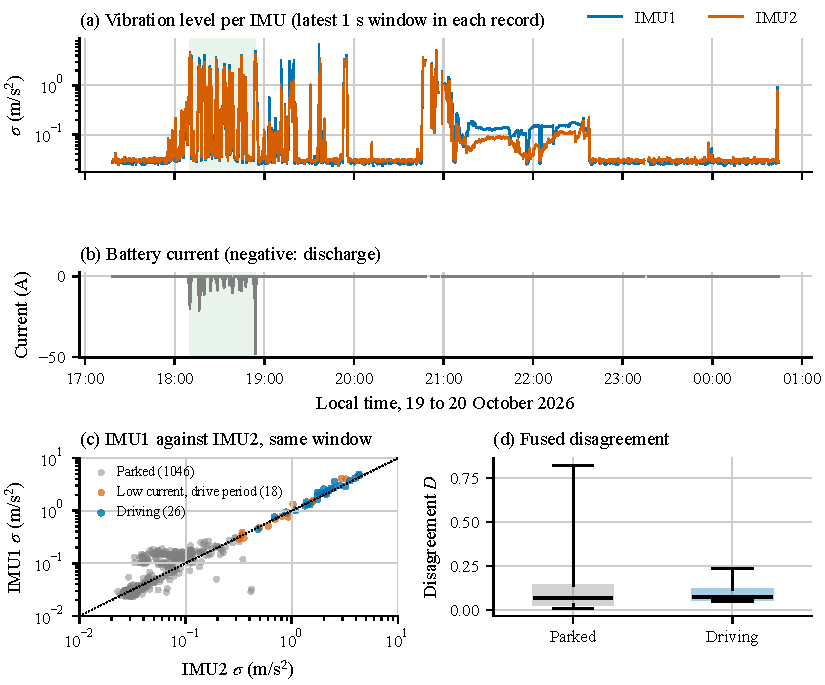
\includegraphics[width=\textwidth]{figures/results/flashlog_run1.pdf}
\caption[Run-1 flash log of the rear unit, boot 109, 19 to 20 October 2026 (\texttt{BenchTest/\allowbreak{}logs/\allowbreak{}flashlog\_\allowbreak{}2026-10-22/\allowbreak{}rear\_\allowbreak{}flash\_\allowbreak{}log\_\allowbreak{}dump.jsonl})]{Run-1 flash log of the rear unit, boot 109, 19 to 20 October 2026 (\texttt{BenchTest/\allowbreak{}logs/\allowbreak{}flashlog\_\allowbreak{}2026-10-22/\allowbreak{}rear\_\allowbreak{}flash\_\allowbreak{}log\_\allowbreak{}dump.jsonl}). (a) $\sigma$ of each IMU in the latest 1\,s window of each record, log scale; (b) battery current; green shading spans the first to the last record with a current above 1\,A. (c) IMU1 against IMU2 $\sigma$ in the same window, dotted line equal; parked, driving, and low-current records within the drive. (d) Disagreement $D$ (Equation~\ref{eq:disagreement}), box at the quartiles, whiskers at the 5th and 95th percentiles. Records are 10 to 58\,s apart; lines break at missing records.}
\label{fig:res-flashlog}
\end{figure}

The battery current reached $-48.03$\,A, against $-46.9$\,A in the recorder, which missed a third of the seconds; the voltage fell from 74.58 to 72.66\,V and the state of charge from 60 to 58\,\%. Driving is taken as a current above 1\,A in magnitude: 26 records, from 18:10 to 18:54, median $-8.1$\,A. Parked is a current within 1\,A and a fused $\sigma$ of at most 0.3\,m/s\textsuperscript{2}: 1,046 records. The other 82, with $\sigma$ above 0.3\,m/s\textsuperscript{2} and no current, are kept apart: 18 fall within the drive, probably coasting or braking, and 64 outside it, between 18:04 and 00:43, when what moved the vehicle or the unit was not recorded. Table~\ref{tab:res-flashlog} and Figure~\ref{fig:res-flashlog} give the result (\texttt{Report/\allowbreak{}figures/\allowbreak{}results/\allowbreak{}flashlog\_\allowbreak{}run1.py}, numbers in \texttt{flashlog\_\allowbreak{}run1\_\allowbreak{}summary.txt}).

\begin{table}[htbp]
\centering
\small
\caption[Ride features per IMU from the run-1 flash log (boot 109): median and, in brackets, 95th percentile of the latest 1\,s window in each record]{Ride features per IMU from the run-1 flash log (boot 109): median and, in brackets, 95th percentile of the latest 1\,s window in each record. Parked: 1,046 records; driving: 26. Units m/s\textsuperscript{2}, crest factor and $D$ none, jerk m/s\textsuperscript{3}.}
\label{tab:res-flashlog}
\begin{tabular}{lrrrr}
\hline
 & \multicolumn{2}{c}{Parked} & \multicolumn{2}{c}{Driving} \\
Feature & IMU1 & IMU2 & IMU1 & IMU2 \\
\hline
RMS & 10.04 (10.08) & 10.34 (10.37) & 10.29 (11.20) & 10.60 (11.34) \\
$\sigma$ & 0.029 (0.162) & 0.031 (0.113) & 2.19 (4.53) & 2.02 (4.22) \\
Peak-to-peak & 0.16 (0.73) & 0.18 (0.50) & 13.9 (21.7) & 11.5 (20.4) \\
Crest factor & 1.008 (1.034) & 1.009 (1.026) & 1.62 (2.09) & 1.51 (1.95) \\
Jerk & 6.4 (35.2) & 6.9 (23.4) & 259 (439) & 248 (382) \\
Fused $\sigma$ & \multicolumn{2}{c}{0.030 (0.131)} & \multicolumn{2}{c}{2.09 (4.40)} \\
Disagreement $D$ & \multicolumn{2}{c}{0.067 (0.825)} & \multicolumn{2}{c}{0.074 (0.241)} \\
\hline
\end{tabular}
\end{table}

While driving, $\sigma$ rose from about 0.03 to a median of about 2\,m/s\textsuperscript{2}, peak-to-peak from about 0.17 to 11 to 14\,m/s\textsuperscript{2}, crest factor from 1.01 to about 1.6 and jerk from about 7 to 250\,m/s\textsuperscript{3}. The two sensors tracked each other closely: while driving, the ratio of IMU1 to IMU2 $\sigma$ had a median of 1.06 (5th to 95th percentile 0.91 to 1.27) and a correlation of 0.97, and $D$ had a median of 0.074 and a 95th percentile of 0.24. Parked, $\sigma$ is near the 0.05\,m/s\textsuperscript{2} floor of Equation~\ref{eq:disagreement}, so $D$ there mostly measures noise. One parked stretch differed: from about 21:00 to 22:40 both sensors read a steady $\sigma$ with no current, median 0.136 for IMU1 and 0.078 for IMU2 against 0.03 at other times; its source was not recorded. Both IMUs were on the rear unit on this day, so their agreement says that they measured the same motion, not how the front and rear of the vehicle compare (Section~\ref{sec:imu-fusion}). The parked RMS of 10.04 and 10.34\,m/s\textsuperscript{2} shows the calibration offset described under R2 above.

These figures come from one session, one 1\,s window in about 23\,s, and only 26 windows identified as driving by current alone; there was no speed (no GNSS antenna) and no marked runs. They show the size of the response and that the two sensors agreed, not its repeatability or its dependence on speed.

\section{Position (R4)}
\label{sec:resx-gnss}

With the corrected parser, the receiver reached a three-dimensional fix 105\,s after a cold start (51\,s in an earlier session), with 23 to 25 satellites and a horizontal dilution of precision of about 0.9 to 1.5. Over 104 fixes the position was a median of 2.7\,m from a phone's position, 95\% within 11.0\,m and at most 12.3\,m away. The phone has an error of a few metres itself, so this is a consistency check, not an absolute accuracy; against the criterion of 10\,m, the median and most fixes pass but the 95th percentile does not. The speed field read 0 to 5.8 while stationary; the manual gives knots, but the readings and their low-speed noise have not been checked against a known speed. The network position (v0.7.3) answered in about 0.7\,s with a reported accuracy of 550\,m.

On the road session of 19 October the receiver reported no fix in any of the 3,464 records, so no position or speed was recorded during the drive. The cause was that no GNSS antenna had been connected to the board, not a fault in the receiver; only the network-based position (about 550\,m accuracy) was available. R4 is therefore untested on the vehicle rather than failed.

Since 22 October a GNSS antenna is fitted; indoors it gave no fix in 6 minutes.

\section{Battery telemetry (R5)}
\label{sec:resx-bms}

After the checksum correction the unit stored 14 consecutive valid records on the vehicle over about 140\,s: 74.78\,V, 0.00\,A and 60\% state of charge (3.12\,V per cell for 24 cells), at $-88$ to $-93$\,dBm, after which the connection was lost. On 16 October, with the telemetry unit moved to within about 2\,m of the pack (Section~\ref{sec:two-sided}), the link held: 60\,\% state of charge, 74.67 to 74.68\,V and 0.0\,A with the vehicle off, each record 0.2 to 1.3\,s old. Before that the laptop had found the unit advertising as ``DB24SA01L24S150ABU'' at $-100$\,dBm, at the edge of reception, which explains the earlier drop-outs. The name gives a 24-cell pack and a 150\,A BMS; 74.7\,V at 60\,\% is 3.11\,V per cell; the chemistry is not confirmed, and lithium iron phosphate, often assumed, would read nearer 3.3\,V at that charge. With the system mounted on the vehicle on 19 October the link held throughout the session, at 60\,\% and 74.57 to 74.58\,V, with each record under 3\,s old. Until the road session the current had not been seen under load.

On the road session the link held throughout. The current reached 46.9\,A under load, the pack voltage fell from 74.6 to 72.8\,V while driving, and the state of charge from 60 to 58\,\%. R5 is partly met: the link held on the vehicle under load, but the voltage has not been compared with a meter.

\section{Hazard sensing (R6 to R8)}
\label{sec:resx-hazard}

Table~\ref{tab:res-camera} summarises the hazard-sensing results and Table~\ref{tab:camera-latency} gives the latency breakdown. With four inference threads and nothing else running (no bridge, no fusion polling, live view not watched; 30 September) the detector ran at 19.5\,frames/s with a median of 102\,ms from sensor readout to result; about 52\,ms of that was readout and the camera's image processing, and 36\,ms inference. With the whole system running on a healthy Raspberry Pi~4 (11 October, from the service's own timing lines) it ran at 14.6 to 14.7\,frames/s, median 118 to 122\,ms, 95th percentile 146 to 148\,ms; the cause of the difference has not been isolated, and these are the figures that represent the rear unit on the vehicle; the front unit on the Raspberry Pi~5 is in Table~\ref{tab:res-camera} and Section~\ref{sec:two-sided}. The three-frame onset adds about two frame intervals, so at the detector an alert is raised about 0.26\,s, or 2.2\,m at 30\,km/h, after an object first appears; the bridge's and dashboard's polling and rendering add an unmeasured delay before the driver sees it. A person was detected with confidence 0.50 to 0.73; only the person class has been confirmed on live frames. These are bench figures with the camera indoors and no objects to track; the number of detections does not change the inference time, but the vehicle's heat and supply may, and detection has not been tested outdoors or in daylight, rain or glare. R7 is met at the detector on the bench, for the person class. R6 is met for the pulse itself, which the camera unit timestamps with a spread of under 0.7\,ms. The offset between the camera's and the telemetry unit's clocks, which aligning the two streams needs, has not been measured; the median interval of 500.06\,ms also means the two clocks run about 120 parts per million apart, about 0.4\,s an hour, so the alignment must fit a drift as well as an offset. Since 22 October the front node's pulse reaches the Raspberry Pi~5 on pin~11 (Table~\ref{tab:res-twonode}); its offset has not been measured either.

\begin{table}[htbp]
\centering
\caption[Hazard sensing on the bench: the Raspberry Pi~4 (the only camera unit until 15 October, the rear unit in the final layout) unless a row names the Raspberry Pi~5]{Hazard sensing on the bench: the Raspberry Pi~4 (the only camera unit until 15 October, the rear unit in the final layout) unless a row names the Raspberry Pi~5.}
\label{tab:res-camera}
\begin{tabular}{|p{6.2cm}|p{7.6cm}|}
\hline
\textbf{Measure} & \textbf{Result} \\ \hline
Camera to telemetry-unit alignment (C6) & Sync pulse median 500.06\,ms, range 499.72 to 500.41\,ms (121 edges, 60\,s) \\ \hline
Detector rate (SSD-MobileNet, 4 threads) & 19.5\,frames/s alone; 17.3 with the live-view server on; 14.6 to 14.7 with the whole system \\ \hline
Sensor readout to result & Alone: 102\,ms median, 120\,ms 95th percentile, 136\,ms maximum. Whole system: 118 to 122\,ms median, 146 to 148\,ms 95th percentile \\ \hline
Alert onset at the detector (3 frames) & about 0.26\,s, 2.2\,m of travel at 30\,km/h (0.2\,s, 1.7\,m alone) \\ \hline
Alert clearing & before the fix, 16 activations in 47\,s for one person; after it, cleared only after 5 empty frames \\ \hline
Time-of-flight sensors (3 $\times$ VL53L0X) & about 31 readings per second each; steady; each confirmed by covering it; not yet checked against a tape. On 12 to 13 October the right sensor started and answered at its address but returned no range (status 4, signal 0 to 13 in 357 readings over 90\,s) while the left and ahead sensors ranged; wiring ruled out, the sensor's aim suspected; after it was adjusted on 14 October it ranged normally (0.63 to 0.67\,m, signal about 70) \\ \hline
Camera and time-of-flight fusion & 29 offline tests pass; first live fused hazard: camera estimate 0.874\,m, time-of-flight 0.096\,m, reported 0.096\,m (before calibration) \\ \hline
YOLO11n, COCO, NCNN, 320 input & 7.9\,frames/s, 175\,ms median readout to result \\ \hline
Approaching-object warning (time to contact from box growth, tracker, ToF closing rate; 15 October) & Implemented; 40 synthetic tests pass (time to contact within 2\,\% at constant speed, no alerts in 5,000 frames of receding, still or jittering boxes); 0.27\,ms per frame on the laptop; not yet run on either Pi or against a real approach (test C11) \\ \hline
Same detector on the Raspberry Pi~5 with the dashboard running (15 October, 60\,s, second OV5647 camera) & 19.2\,frames/s; readout to result 51 to 54\,ms median, 61 to 63\,ms 95th percentile (inference 28\,ms median); CPU 64 to 73\,\%, 53 to 54\,\textdegree C, no throttling; one person alert raised and cleared \\ \hline
Pothole model, run 1 & mAP@50 0.597 on its own test set; 0.000 on South African frames \\ \hline
Pothole model, run 2 (road-band tiles) & mAP@50 0.714 at 640 and 0.566 at 320, on validation tiles \\ \hline
Pothole path inside the detector (C10) & Found the pothole in a test picture (confidence 0.63); detector 13.9\,frames/s at one run per 4\,s, 10.9 to 13.3 at higher rates or with more threads; off by default \\ \hline
\end{tabular}
\end{table}

\begin{figure}[htbp]
\centering
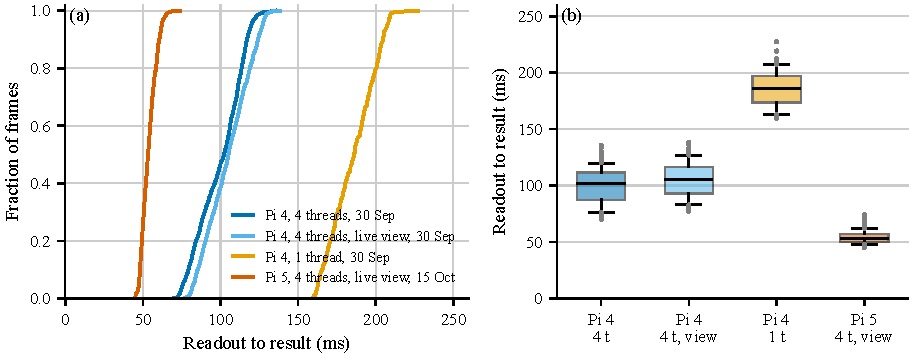
\includegraphics[width=\textwidth]{figures/results/detector_latency.pdf}
\caption[Detector latency from camera readout to detection result, per frame, for 60\,s runs of the TensorFlow Lite detector (\texttt{detect.tflite}, 300$\times$300 input, 640$\times$480 camera stream)]{Detector latency from camera readout to detection result, per frame, for 60\,s runs of the TensorFlow Lite detector (\texttt{detect.tflite}, 300$\times$300 input, 640$\times$480 camera stream). (a) Cumulative distribution; (b) box plots with the box at the quartiles, whiskers at the 5th and 95th percentiles and dots beyond them. Pi~4 runs on 30 September: four threads (1161 frames, 19.5 frames/s), four threads with the live view open in the Pi's browser (1031 frames, 17.3 frames/s), one thread (419 frames, 7.0 frames/s). Pi~5 run on 15 October: four threads with the live-view server running (1151 frames, 19.2 frames/s). Data from the detector's per-frame timing CSV files.}
\label{fig:res-latency}
\end{figure}

Figure~\ref{fig:res-latency} compares the per-frame time from sensor readout to detection result. On the Pi~4 with four inference threads the median was 102\,ms (95th percentile 120\,ms, 1161 frames) and 105\,ms with the live view open (127\,ms, 1031 frames); with one thread it rose to 186\,ms (207\,ms, 419 frames) as inference went from 36 to 126\,ms. The Pi~5 on 15 October had a median of 53\,ms and a 95th percentile of 62\,ms over 1151 frames, with inference at 28\,ms and queue wait at 18\,ms against 52\,ms on the Pi~4. The 11 October whole-system log on the Pi~4 (bridge, fusion and preview running) recorded only per-interval summaries, median 118 to 122\,ms and 95th percentile 146 to 148\,ms, so it is not plotted.

The time-of-flight stand-ins answered and each responded to a fingertip in the right order (centre 267 to 300\,mm and right 24 to 38\,mm on the bench; left 8190, the code for no target), so the first part of R8 is met; their accuracy against a tape and the fusion validation (test C9) have not been run, so the rest of R8 is outstanding. The first live fused hazard shows the matching working and how far the uncalibrated camera distance can be wrong at close range. The fusion's sensor directions and the camera's focal length are still defaults.

On the road session (17:15 to 19:10) the front detector raised 1,342 alerts: people 815, of which 366 were marked approaching, and cars 513, of which 261 were approaching. The rear detector raised 741, from its own log: people 514 (183 approaching), cars 201 (36 approaching) and 26 other vehicles. Whether each alert was correct has not been checked against video.

Not measured by the time of writing: the fusion validation C9 (distance error against a tape at 0.5, 1.0 and 1.5\,m), the camera's focal length (begun on 19 October, test C5, not finished) and the pothole model's held-out test score. Until they are done the distance bands and fused distances are indicative only.

\section{Telemetry, logging and recovery (R9, R10)}
\label{sec:resx-telemetry}

The unit connected to the broker at the first attempt and published 47 times with no failures; a requested reconnection completed in 0.4\,s. With the modem's radio switched off for 60\,s, the firmware detected the loss from the modem's report 0.8\,s after the radio went off, or after three failed publishes at 20.7\,s, and retried after 30 and then 60\,s. In v0.5.0 it reconnected 36\,s after the radio returned, waiting for its next retry although data were back within 2.4\,s; v0.5.3 reconnected about 5\,s after. Logging continued throughout. A full read-back recovered all 6,020 stored records (2.2\,MB, about 16.7 hours at one record per 10\,s) after four passes; 5,545 were not valid JSON because of \texttt{nan}, and after the v0.6.3 substitution all 6,020 parse.

Synchronisation with the database was tested with v0.7.4 (test T15, 11 October, indoors, public test broker; Table~\ref{tab:res-sync}). Every record was stored once, but 24 only after a backfill from the unit's log: two published while the ingest was restarted, the rest before an ingest fault found during the test was fixed (its persistent session on the broker stopped delivering while still connected; such sessions are now opt-in). The public broker acknowledges a record with no subscriber present and does not queue it, so on this broker reading the log back is the safety net. R9 is met on the bench, including the database.

Figure~\ref{fig:res-t15} shows the backlog during T15. With the radio off for 600\,s the backlog grew by one record every 10\,s to 60 records, MQTT reconnected 5.2\,s after the radio was switched back on, and the backlog was cleared 37.9\,s later. On the server side the 60 replayed records arrived over 37.3\,s (1.6 records/s), and the database held all 112 records expected for the boot (sequence 65 to 176) with no duplicates and none missing.

The dashboard line (v0.7.0) delivered 40 lines in 40\,s with no gap in the sequence numbers, every line valid JSON and at most 272 bytes, with both IMUs at 200\,Hz and no drops. Through the bridge on the Raspberry Pi~4 the record reached a laptop, not yet the Raspberry Pi~5, 0.37\,s old with no malformed lines, and opening the port did not reset the telemetry unit; the pre-test check on 4 October found the record 0.5\,s old and the telemetry answering in 18\,ms. In a longer bench run (12 to 13 October, 4.7 hours, v0.7.4 with the modem and the database sync active) the bridge counted 858 unusable dashboard lines among 9,229 lines read (9.3\,\%); the cause has not been found. On 16 October it fell to about 2\,\% (1.9 to 2.8\,\%), then rose to 10 to 11\,\% once the battery-management link was active, with the Raspberry Pi~4 under-voltage at the same time (Section~\ref{sec:inv-power}). A skipped line delays the dashboard by a second; the unit's own log and the uplink are not affected. On the road session a third of the per-second records did not reach the recorder for the same reason (Section~\ref{sec:res-acq}). Since 21 October the record travels over a wired UART instead of USB (Section~\ref{sec:pi-link}): none of the first 2,489 lines was bad, and in the 62-minute soak of 22 October the bridge read 3,720 lines in 3,720\,s with none bad. The front node's stream reached the Raspberry Pi~5 over USB with no bad CRC (Table~\ref{tab:res-twonode}). R10 is met on the bench over the wired link; on the vehicle it is untested since the change.

\section{Driver display (R11, R12)}
\label{sec:resx-display}

Run on a laptop inside a copy of the dashboard's code, against the live detector on the Raspberry Pi~4 (1 October), the camera page showed video 0.6\,s after it was opened and decoded 14.2\,frames/s against the detector's 14.8, with no gap longer than 0.22\,s; with a person in front of the camera it listed a red ``Person, Immediate'' alert 0.5\,s after the page was opened with the person already in view (not an onset latency), and it switched to its offline state within a second of the detector stopping; the person stayed in view, so clearing on the page was seen only in the offline test and when the camera stopped, although the detector's log shows person alerts both raised and cleared. In live-only mode, run offscreen on a laptop against a simulated bridge (3 October), every page showed ``-{}-'' or ``Unavailable'' with the bridge down and never a simulated value, and the dashboard returned to the no-data state, not to simulation, when the bridge stopped. In an offscreen run of the whole integrated dashboard on the Raspberry Pi~5 against the live bridge (6 October), the Sensors page showed the ahead sensor at 0.43\,m in red, the right at 0.69\,m in amber and the left with no reading, and the banner appeared over the driving page; the page's use by touch had not been checked at the time. Reading the touch controller during 25 taps, the panel reported contact together with the first position in every tap, so it adds no measurable delay; the taps lasted 200 to 640\,ms and the buttons act on release, and the processor was idle (load average 0.04). R11 is partly met: alerts were seen to clear only in offline runs. R12, the glance demand, has not been measured. Its precondition, legibility, was measured on 24 October without a participant (\texttt{BenchTest/\allowbreak{}legibility\_check.py}, output in \texttt{BenchTest/\allowbreak{}logs/\allowbreak{}legibility\_2026-10-24}): the deployed dashboard was run offscreen at 1280 by 800 with the deployed settings, every page shown in turn, and every visible label's capital height taken from the font's own metrics (\texttt{QFontMetricsF.capHeight}); text painted directly (the speed digits and the alert banner) was measured on the Raspberry Pi~5's screenshot of 23 October. With 0.170\,mm per pixel and an assumed eye distance of 0.70\,m (to be measured from the seat), ISO~15008's 20 and 16 arc minutes are capitals of 24.0 and 19.2\,px (20.5 and 16.4\,px at 0.60\,m). Measured: speed digits 100\,px (83.5 arc minutes); alert banner 11\,px (9.2); page titles 15.4\,px (12.9); labels a median of 11.2\,px (9.3), with 4 of 110 distinct labels at 16 arc minutes or more, all of them on the reverse-camera page. Of 26 enabled buttons the smallest side has a median of 10.9\,mm (range 7.5 to 61.2), 25 are at least 10\,mm and 5 at least 17.5\,mm, the size up to which touch keys kept improving \cite{kim2014touchkey}. The speed is far larger than needed; the warnings, labels and most touch targets are smaller than the cited figures.

Alert onset to screen on the Raspberry Pi~5 has not been measured, and no glance study is planned: no person takes part as a subject (Section~\ref{sec:ethics}), so R12 is left for future work.

\section{Integration and power}
\label{sec:resx-power}

All telemetry-unit subsystems ran together on the target board, and the chain from the telemetry unit through the Raspberry Pi~4 to the dashboard on the Raspberry Pi~5 ran on the bench. The under-voltage that throttled the Raspberry Pi~4 through the bench work, and held the detector at 6.1\,frames/s on 4 October, was traced to the telemetry unit's modem on its USB port (Section~\ref{sec:inv-power}). The Pi reached 81\,\textdegree C without a fan and 48 to 66\,\textdegree C with one.

On 19 October the whole system was mounted on the vehicle and checked in the lab. Both cameras and detectors ran (front 17.5 to 22.0\,frames/s, 53 to 102\,ms; rear 14.4 to 14.5\,frames/s, 126 to 151\,ms, slower while the Raspberry Pi~4 was throttled). Both time-of-flight boards answered, both IMUs held 200\,Hz with no drops, and the battery link reported on the vehicle. The Ethernet link ran at 1000\,Mb/s with a 0.25\,ms round trip, and the recorder on the Raspberry Pi~5 received all four sources at 2\,Hz. The Raspberry Pi~4 logged 11 to 16 under-voltage warnings per boot with the telemetry unit still on its USB port, and both computers restarted during the mounting work (Section~\ref{sec:inv-power}). Table~\ref{tab:power-budget} gives the power budget against the 72\,V pack (GA~5). Only the Raspberry Pi~5 figure is measured, from its own power-management readings on 14 October with the dashboard running (2.2 to 3.0\,W on its internal rails, before it took on the front camera, detector and time-of-flight board on 15 October, so its share in the final layout is higher than shown); the rest are estimates from datasheets and published bench figures, to be replaced by inline USB meter readings. On the same day the Raspberry Pi~4, with the detector using three of its four cores, reported that its supply had fallen below the under-voltage threshold since boot (\texttt{get\_throttled} 0x50000), so its present supply is not adequate.

\begin{table}[htbp]
\centering
\small
\caption[Power budget of the added electronics at 5\,V, and the draw on the 72\,V pack through a DC-DC converter of about 88\,\% efficiency]{Power budget of the added electronics at 5\,V, and the draw on the 72\,V pack through a DC-DC converter of about 88\,\% efficiency. Typical is the steady draw while driving; peak is the worst short burst, not all at once.}
\label{tab:power-budget}
\begin{tabular}{|p{5.6cm}|p{1.5cm}|p{1.3cm}|p{5.2cm}|}
\hline
\textbf{Load} & \textbf{Typical (W)} & \textbf{Peak (W)} & \textbf{Source} \\ \hline
Raspberry Pi~5, dashboard (measured before the front camera unit was added) & 4.0 & 8 & Measured 2.2 to 3.0\,W on the rails, plus input conversion and USB \\ \hline
10.1\,in display, full backlight & 5.0 & 6 & Estimate; to measure \\ \hline
Raspberry Pi~4 with camera, fan and three ToF sensors, detector running & 6.8 & 8 & Estimate from published full-load figures (about 6.4\,W) plus the camera, fan and sensors \\ \hline
ESP32-S3, A7670 modem (with GNSS) and two IMUs & 1.0 & 9 & Estimate; the modem's transmit bursts of up to about 2\,A are the peak, and the cause of the brown-out in Section~\ref{sec:inv-power} \\ \hline
SEN55 (planned) & 0.4 & 0.5 & Datasheet \\ \hline
\textbf{Total at 5\,V} & \textbf{17} & \textbf{31} & \\ \hline
\textbf{From the 72\,V pack} & \textbf{20 (0.27\,A)} & \textbf{35 (0.5\,A)} & At 88\,\% converter efficiency \\ \hline
\end{tabular}
\end{table}

At about 20\,W the added electronics use 20\,Wh per hour, 160\,Wh over an eight-hour shift. Against a 7.2\,kWh pack, the figure the team's dashboard uses (not confirmed; the BMS's name gives 24 cells but not the capacity), that is 0.28\,\% of the pack per hour and 2.2\,\% per shift, and about 0.8\,\% of the motor's rated input of 2.5\,kW. The draw is small while driving but not when parked: left on, the full system would empty the same pack in about 15 days, so it must switch off with the vehicle, leaving at most the telemetry unit (about 1\,W) on. The converter must accept the pack's whole voltage range, about 60 to 88\,V for its 24 lithium iron phosphate cells (R5 above), and be rated to at least 100\,V for transients, and deliver at least 40\,W at 5\,V for the peaks, with a fuse of about 2\,A on its 72\,V input.

On the road session the recorder on the Raspberry Pi~5 ran for 108.6 minutes without the laptop and did not restart while driving, and the front sources were recorded throughout. The rear unit answered it until 18:49:13, just after the last driving segment, and not for the last 15 minutes (1,785 failed requests), although the rear detector kept logging its alerts until 19:02; the cause was not recorded. Before that the rear data had one gap, of 409\,s, before the drive, and a third of its seconds had no new record (Section~\ref{sec:res-acq}).

Not measured by the time of writing: the inline current of the display, the Raspberry Pi~4 and the telemetry unit, which would replace the estimates in Table~\ref{tab:power-budget}, and the pack's capacity, which the vehicle team has not confirmed.
